\section{Results}
\label{Spline_1}

\subsection{Results}
 
 In our case we simulated the results and found following outputs.
Plotting the second order curve for given data of IMU with just least square method. We get

\begin{figure}
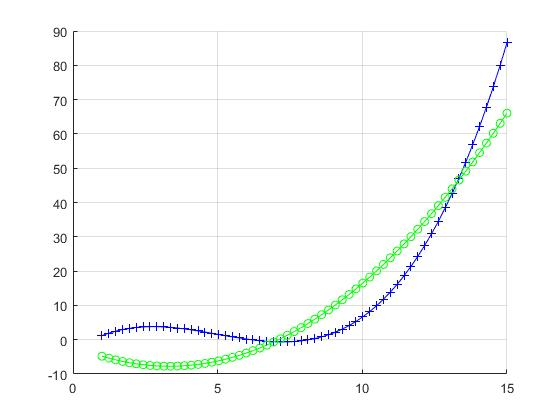
\includegraphics[width=\textwidth]{./figures/lsm.jpg}
\caption{In this case Blue is actual curve traced by IMU this are points with noise.And green is plotted curve. With least square method.}
\end{figure}

Then according to the paper we fused data of camera and IMU so we get following graph.

\begin{figure}
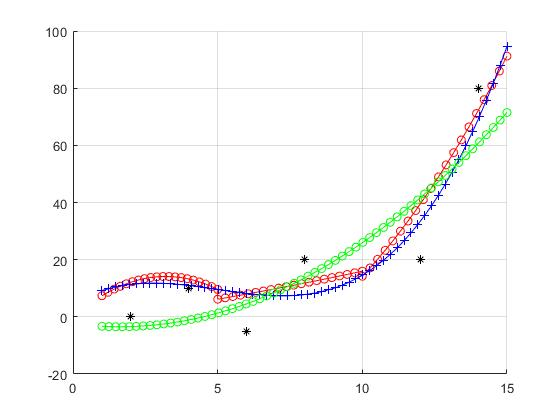
\includegraphics[width=\textwidth]{./figures/AllOutput.jpg}
\caption{Multiple result Graph}
\end{figure}

Here we have 3 curved fitted as shown as red which gives better results and it also uses data of camera shown with black dots. So here according to the above formula scale factor of different section is different it is according to the quality of reading by camera.
For example, in our case 
\begin{equation}
\lambda_1=0.5 ,\lambda_2=0.5 ,\lambda_3=0.1
\end{equation}

In 3rd section camera readings were not accurate so taken into smaller scalar value. This camera data further improved the result. And we get minimum error and good fit. With the given spline fitting method.

So if we look into different of error with traditional Least square method with Jung and Taylor method. It gives good results. Almost we get the same curve.

\begin{figure}
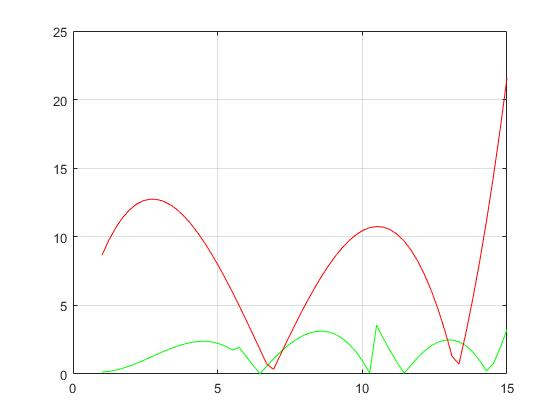
\includegraphics[width=\textwidth]{./figures/ErrorC.jpg}
\caption{A. Red curve for method with one curve and least square method. 
B. Green curve is using the given method by Jung and Taylor.}
\end{figure}

This graph has error comparison with and without Jung and Taylor method of split curve fitting and scaling camera input.
So it is better to follow the given first method in the paper. It results into considerable reduction in error. which is clearly seen in graph.
  